\documentclass[a4paper,29.6pt]{article}
%\documentclass[a4wide]{scrreprt}
\usepackage{graphicx}
%\usepackage{hyperref}
%\usepackage{palatino}
%\usepackage{hyperref}

%\parskip 7.2pt % sets spacing between paragraphs

%\renewcommand{\baselinestretch}{1.5} % Uncomment for 1.5 spacing between lines

%\parindent 0pt % sets leading space for paragraphs

\title {Project Report \\ Sensor Module Interfacing \\[10pt] Task: RFID Module Interfacing \\[25pt] Team members }
\author {Chayatan \and Mukilan A \and Shanthanu Senguptha}

\begin{document}
\maketitle
\begin{center}
\begin{large}
Under the guidance of\\
\textbf{Prof. Kavi Arya\\and\\Parin Chedda}\\
\vspace{0.5in}
\end{large}
\end{center}
\begin{center}

\includegraphics[scale=0.32]{images/iitb}
\end{center}
\begin{center}
\begin{large}
Embedded and Real-Time Systems Laboratory \\
Department of Computer Science and Engineering \\
Indian Institute of Technology \\
Bombay \\
\end{large}
\end{center}
%\pagenumbering{roman} % Roman page number for toc
%\setcounter{page}{1} % Make it start with "ii"

\newpage
\tableofcontents
\newpage

\begin{abstract}
The project aims at Constructing a simple circuit and choosing the appropriate protocol to interface RFID sensor Module to the FireBird V Robot. in the present scenario the most common problem faced on this planet is the identification problem. where ever you go people ask your identity proof. Nowadays we need to take permission to carry our belongings too. in order to track this problem we henceforth came up with this idea of using RFID reader and RFID tags. 
\end{abstract}

\section{Introduction}

\begin{large}
\hspace{.5in}Radio Frequency Identification (RFID) is a technique that uses short range radio frequency transmissions to read and write data to an RFID tag. This tag can be powered by an electromagnetic field, eliminating the requirement of using of batteries or mains power for the device. This device is most commonly used as a way to uniquely identify a specific device or object.
\\\\
The detail description of RFID reader, different types of tags, interfacing circuit, appropriate C code and its major applications in todays world is explained below.\\

\end{large}
\begin{center}
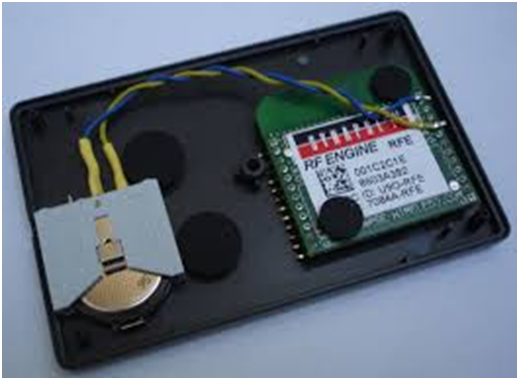
\includegraphics[scale=0.5]{first}
\end{center}


\newpage

\subsection{RFID Reader}
\begin{small}
The EM-18 RFID Reader module operating at 125 kHz is an inexpensive solution for your RFID based application. The Reader module comes with an on-chip antenna and can be powered up with a 5V power supply. 
Power-up the module and connect the transmit pin of the module to receive pin of the microcontroller. Show your card within the reading distance and the card number is thrown at the output. Optionally the module can be configured for also a weigand output.\\


\subsection{RFID Tags}
\begin{small}
Originally, RFID tags were used to track large items, like cows, railroad cars and airline luggage that were shipped over long distances. These original tags, called inductively coupled RFID tags, were complex systems of metal coils, antennae and glass.
Capacitively coupled tags were created next in an attempt to lower the technology's cost. These were meant to be disposable tags that could be applied to less expensive merchandise and made universal as bar codes. Capacitively coupled tags used conductive carbon ink instead of metal coils to transmit data. The ink was printed on paper labels and scanned by readers.
Newer innovations in the RFID industry include active, semi-active and passive RFID tags. These tags can store up to 2 kilobytes of data and are composed of a microchip, antenna and, in the case of active and semi-passive tags, a battery. The tag's components are enclosed within plastic, silicon or sometimes glass.
Active and semi-passive RFID tags use internal batteries to power their circuits. An active tag also uses its battery to broadcast radio waves to a reader, whereas a semi-passive tag relies on the reader to supply its power for broadcasting

\end{small}


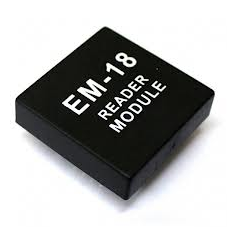
\includegraphics{em18}
\cite{em18}\and
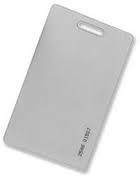
\includegraphics[scale=0.38]{tag}


\hspace{1in}Fig1\hspace{2.2in}Fig2
\end{small}

\subsubsection{Passive Tags}
\begin{small}
In this experiment we are exclusively dealing with passive tags.\\
A \textbf{ passive tag }is an RFID tag that does not contain a battery within it. The power is supplied by the reader. When radio waves from the reader are encountered by a passive RFID tag, the coiled antenna within the tag forms a magnetic field. The tag draws power from it, energizing the circuits in the tag. The tag then sends the information encoded in the tag's memory.
\newpage
\textbf{The advantages of a passive tag are:}\\ 
\begin{itemize}
\item	The tag functions without a battery; these tags have a useful life of twenty years or more. 
\item	The tag is typically much less expensive to manufacture 
\item	The tag is much smaller (some tags are the size of a grain of rice).
\item These tags have almost unlimited applications in consumer goods and other areas.
\end{itemize}
 
\textbf{The major disadvantages of a passive RFID tag are: }
\begin{itemize}
\item	The tag can be read only at very short distances, typically a few feet at most. This greatly limits the device for certain applications. 
\item	It may not be possible to include sensors that can use electricity for power. 
\item	The tag remains readable for a very long time, even after the product to which the tag is attached has been sold and is no longer being tracked.
\end{itemize}
 

\end{small}

\section{Working of RFID Module}
A  passive  RFID tag  consists  of  three  parts:  an antenna,  a  semiconductor  chip  attached  to  the  antenna,  and  some  form  of encapsulation. The tag reader is responsible for powering and communicating with a tag. The tag antenna captures energy and transfers the tag’s ID (the tag’s chip coordinates this process).  The encapsulation maintains the tag’s integrity  and protects  the  antenna and  chip  from  environmental  conditions.\\ Ensure the following features are taken care before using.\\
The reader reads the tag and transmits the information at 9600 baud rate, 8bit data with one stop bit and no parity bits. The working of the RFID can be checked on serial terminal. After this checking is successful, interface it to the firebird or any other microcontroller.

\subsection{Features of RFID Reader EM-18}
\begin{itemize}
\item	5V supply
\item	125kHz read frequency
\item	9600bps TTL and RS232 output
\item	Magnetic stripe emulation output
\item	10 cm read range
\end{itemize}

\newpage

\section{Circuit Connection Details}
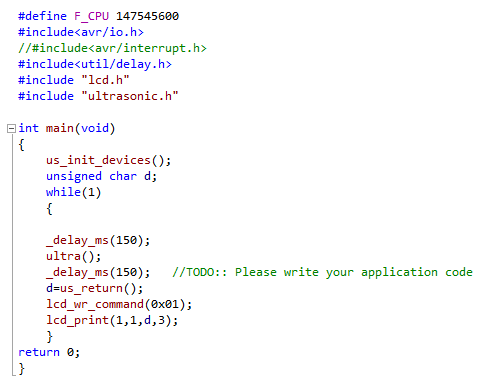
\includegraphics[scale=0.4]{app}
\cite{app}

\begin{enumerate}
\item	Make sure the VCC and GND pins are properly connected.
\item	Connect the SEL pin to VCC
\item	Now connect the TX pin of EM-18 reader to the RX pin of AVR microcontroller. This pin is available on the expansion slot. We are actually using the USART3 of the microcontroller. Its pin 46 female slot on the expansion slot. 
\item	Program the controller to receive according to the above explained features.
\item	Display the read information on LCD

\end{enumerate}
*please note that pin no.46 is the RX pin on the expansion slot available on FireBird V
\newpage
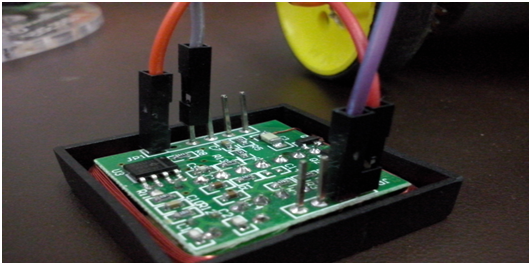
\includegraphics[scale=0.5]{conn}\and
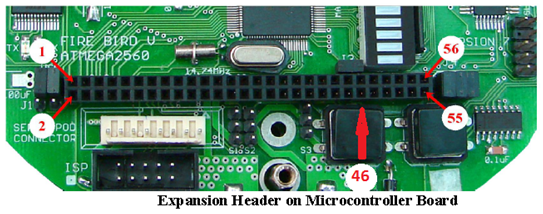
\includegraphics[scale=0.4]{exp}


\hspace{1in}Fig3\hspace{2.5in}Fig4
\\Fig3 shows the necessary connection to be done on the EM-18 reader module.\\
Fig4 shows the the RX pin of the microcontroller on the expansoion slot.

\section{ Serial Terminal }
A sample output of the EM-18 reader as seen on the serial terminal\\
Note: Please see the tutorial on how to check the output on the Serial Terminal.\\\\
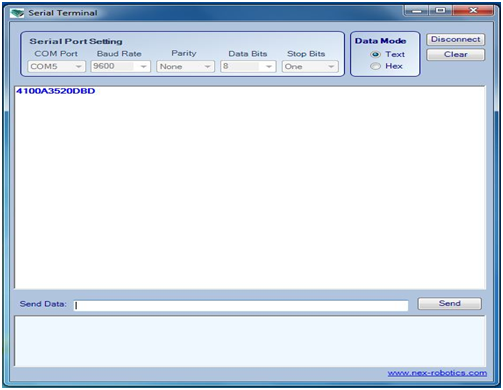
\includegraphics{serial}


\newpage
\section{The C code highlights}
\begin{small}
This code tries interpret the information transmitted from the RFID reader module and keeps it in the character array format which is suitable for further processing.\\\\
Interrupt Service Routine is called whenever the Tag is brought near to the reader causing an interrupt.\\
This routine stores the 12 bytes serially transmitted information, in an array called ‘arr’ which is of size 12 bytes. A counter is used to check whether 12 bytes has arrived or not. If the counter is 12, then it is reset to zero and the content of the array is displayed on the LCD screen.\\\\
The rf\_init\_devices() is  an user defined function which is used to initialize all the devices such as UART, lcd and configuration of all the ports.\\\\
The rf\_display() function is a user defined  function to store the data in ‘arr’ and display the contents of  the ‘arr’ array on the lcd screen.\\\\
The rf\_return() function is used to return the read value whenever it is needed and this function is helpful to compare a particular value with the instantaneous data.\\\\
The rf\_init\_devices,  rf\_display() and rf\_return() functions are used in the main function of the ‘rfiddb’ project file to create a database and for comparison.

\end{small}
\section{Sample output on RFID}
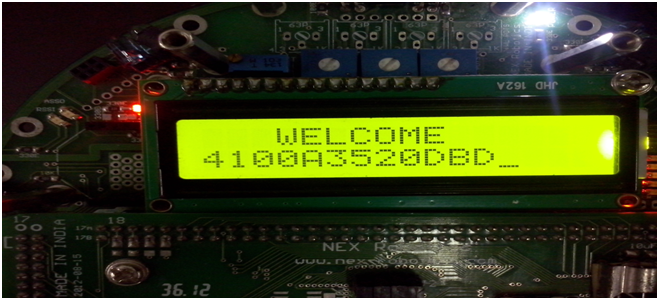
\includegraphics[scale=0.5]{lcd}

\newpage
\section{Application program}
\begin{small}
\textbf{Demonstration of how an RFID reader and RFID tags can be used to build an application}\\
Here is a small application where in we are receiving the information and checking if the particular person having a Tag is a valid user or an invalid user.\\
Here we have made use of the created header file ‘rfid.h’ and we have used the rf\_display and rf\_return function to display and check whether he or she is having a valid Tag. Correspondingly he or she can be permitted or discouraged to enter a building or use a particular device.\\\\
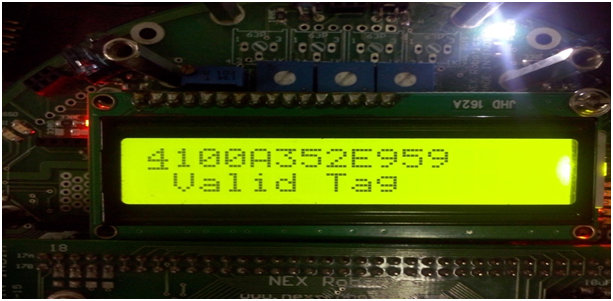
\includegraphics[scale=0.5]{lcd2}
\end{small}
\section{RFID Applications}
\begin{small}
We all know RFID tags are largely used to store students and teacher’s databases. It can store the person’s data such as his or her address, phone and many more. Apart from this, RFID tags can be used instead of barcodes under special conditions.\\\\
RFID tags are an improvement over bar codes because the tags have read and write capabilities. Data stored on RFID tags can be changed, updated and locked. Some stores that have begun using RFID tags have found that the technology offers a better way to track merchandise for stocking and marketing purposes.\\\\
In addition to retail merchandise, RFID tags have also been added to transportation devices like highway toll pass cards and subway passes. Because of their ability to store data so efficiently, RFID tags can tabulate the cost of tolls and fares and deduct the cost electronically from the amount of money that the user places on the card. Rather than waiting to pay a toll at a tollbooth or shelling out coins at a token counter, passengers use RFID chip-embedded passes like debit cards.

\end{small}

\newpage
\begin{thebibliography}{99}
\bibitem{em18} \url{http://entesla.com/image/cache/data/Products/RF/em-18\_rfid\_module-900x900.jpg}
\bibitem{app}
\url{http://entesla.com/image/data/Products/RF/EM-18\%20application%20circuit.jpg}

\end{thebibliography}
\end{document}